%=============================================================================
%  FYP Project Proposal  --  Yuxuan LI (20616316)
%
%  Compiles with:  pdflatex -> bibtex -> pdflatex -> pdflatex
%  TeX Live is at /Library/TeX/texbin (may not be on PATH).
%
%  Structure follows the FYP specification: cover page, background and
%  motivation, aim and objectives, work plan, bibliography.
%  Length limit: 2,000 words excluding the cover page.
%=============================================================================
\documentclass[11pt,a4paper]{article}

\usepackage[utf8]{inputenc}
\usepackage[T1]{fontenc}
\usepackage[a4paper,margin=2.5cm]{geometry}
\usepackage{amsmath,amssymb}
\usepackage{booktabs}
\usepackage{enumitem}
\usepackage{microtype}
\usepackage{tikz}
\usepackage[numbers,sort&compress]{natbib}
\usepackage[hidelinks]{hyperref}

% paragraphs: no first-line indent, one blank line between them
\setlength{\parindent}{0pt}
\setlength{\parskip}{\baselineskip}

\setlist{nosep,leftmargin=1.3em}
\renewcommand{\bibfont}{\footnotesize}

\begin{document}

%------------------------------------------------------------------ cover page
\begin{titlepage}
\centering
\vspace*{0.8cm}

{\large University of Nottingham Ningbo China\par}
\vspace{0.25cm}
{\large Department of Computer Science\par}

\vspace{2.6cm}
{\Huge\bfseries Final Year Project Proposal\par}

\vspace{1.6cm}
\rule{\textwidth}{0.4pt}
\vspace{0.9cm}

{\LARGE\bfseries Multi-Objective Optimization for\\[0.35em]
 Large-Scale Neural Solver Deployment\\[0.35em]
 for Combinatorial Optimization\par}

\vspace{0.9cm}
\rule{\textwidth}{0.4pt}

\vspace{2.8cm}
{\large
\begin{tabular}{@{}r@{\hspace{1.2em}}l@{}}
\textbf{Name:}              & Yuxuan LI \\[0.55em]
\textbf{Student ID:}        & 20616316 \\[0.55em]
\textbf{Email:}             & scyyl36@nottingham.edu.cn \\[0.55em]
\textbf{Programme of Study:} & BSc Computer Science and Artificial Intelligence \\[0.55em]
\textbf{Supervisor:}        & Ruibin BAI \\
\end{tabular}\par}

\vfill
{\large 9 October 2026\par}
\vspace{0.6cm}
\end{titlepage}

%=============================================================================
\section{Background and Motivation}
%=============================================================================

Combinatorial optimization problems such as the travelling salesman problem (TSP)
and the capacitated vehicle routing problem (CVRP) underpin logistics, scheduling
and network design. Neural combinatorial optimization (NCO) now solves them
competitively with classical heuristics, through constructive models
\citep{kool2019attention,kwon2020pomo}, heatmap-and-search methods
\citep{joshi2019gnn,sun2023difusco}, learned improvement operators
\citep{ma2021dact,hottung2022eas} and decomposition \citep{duan2023htsp,ye2024glop}.
These are almost all research results. What a trained solver costs to \emph{run},
as opposed to how good its tours are, has received little systematic attention.
This project addresses that gap. Its subject is the deployment-time inference
efficiency of NCO solvers: where the cost of a fixed, trained solver goes when it
is executed repeatedly in production, and how much of that cost can be removed
without retraining the model.

Reporting conventions obscure the question. A typical paper quotes a single pair
of numbers --- solution quality and runtime --- measured on one accelerator, with
runtime treated as an undifferentiated wall clock. That conceals how inference
time decomposes into arithmetic, kernel launch, host--device synchronisation and
Python dispatch; how much of it is recoverable by the techniques a deployment
engineer actually controls; and how the answers change with the number of
instances served, the degree of concurrency and the length of the run. The
magnitude is not academic: on TSP-1000, POMO with 8-fold augmentation is reported
at a 40.57\% optimality gap and 8.5 minutes, against 3.168\% and 1.6 minutes for
a greedy heatmap-plus-search method \citep{luo2024icam}. A difference that large
decides whether a method is deployable at all, yet it becomes visible only when
quality and latency are reported together across scales.

Where inference cost is addressed at all, the treatment is algorithmic rather
than systemic. StruDiCO reports a $3.5\times$ speedup and 70\% memory reduction by
restructuring the denoising process \citep{wang2025strudico}, and Fast T2T reaches
order-of-magnitude gains by replacing iterative training-to-testing solving with a
consistency objective \citep{li2024fastt2t}. Both redesign the model; neither asks
what a \emph{fixed} solver costs to run, or how much of that cost falls to
compilation, batching, reduced precision and memory management --- the levers
available without touching the model. One level further out, the Amortized
Efficiency Threshold (AET) asks how many instances must be served before a neural
solver's training energy is repaid by its per-instance inference advantage,
reporting a crossover near $1.58\times10^{5}$ instances at $n{=}20$
\citep{aet2026}. That result is validated at a single scale on a single hardware
configuration, so whether the threshold rises, falls or inverts under
deployment-scale conditions is unknown.

My reading is that this gap is structural rather than a matter of further tuning.
In the NCO literature ``large-scale'' almost always denotes large instance size;
for deployment the binding constraint is usually how many instances arrive, how
many are served concurrently, and how long the service runs. A survey of analytics
and machine learning in vehicle routing likewise identifies the distance between
what learning-based methods demonstrate in research and what operators can run in
practice as a recognised open problem \citep{bai2023analytics}. I will therefore
characterise neural solver cost along that deployment axis, holding the solver
fixed rather than proposing a new one, so that the measurements describe a system
rather than a contribution. The platform is held fixed as well: every measurement
is taken on a single NVIDIA GPU workstation, which isolates solver configuration
from platform variation and makes the measured quality--latency trade-off a
property of the solver rather than of the machine that ran it. Generality is
tested instead across solver families --- constructive, heatmap-based and
improvement methods --- which asks the same deployment question of three different
kinds of model.

%=============================================================================
\section{Aim and Objectives}
%=============================================================================

\paragraph{Aim.} The aim of this project is to characterise where inference cost
is spent in neural combinatorial optimization solvers at deployment scale, to
quantify how much of that cost is recoverable through system-level optimisation,
and to derive a decision rule that identifies the cost-optimal solver
configuration for a given workload and solution-quality constraint.

\paragraph{Objectives.} The following objectives specify the individual aspects
that must be delivered to achieve the aim.

\begin{enumerate}[label=\textbf{O\arabic*.},leftmargin=2.6em]

\item \textbf{Establish a reproducible measurement environment.} Pin the
reference codebase to one revision and hold it read-only; generate instance sets
once, with fixed seeds, and reuse them across every run; and repeat a fixed
calibration workload at the start of every measurement session, so that drift in
clocks, thermals or driver state is detected rather than mistaken for an effect
of the code.

\item \textbf{Characterise where inference time is spent.} Profile a reference
workload to attribute time to arithmetic, kernel launch, host synchronisation and
Python dispatch, and determine how that attribution migrates as instance size,
batch size and decoding budget increase.

\item \textbf{Quantify how much of the inference cost is recoverable.} Measure the
effect of compilation, batching and reduced precision against an eager baseline,
one intervention at a time, and then restructure the autoregressive decode loop,
whose per-step host synchronisation to test a termination condition lies outside
any compiled subgraph. Establish whether the total headroom grows or shrinks with
instance size.

\item \textbf{Formulate deployment as a multi-objective problem.} Trace the
Pareto front over solution quality and latency under a quality constraint, and
derive the decision rule the aim specifies.

\item \textbf{Test the result beyond the base setting.} Repeat the key
measurements on a second problem family (TSP to CVRP) and across solver families;
compute the Amortized Efficiency Threshold against a strong heuristic baseline,
charging the full training cost, and test how the threshold varies with instance
size, batch size and model family. Identify which conclusions transfer and which
reverse.

\end{enumerate}

%=============================================================================
\section{Project Plan}
%=============================================================================

The project runs for six months, October 2026 to March 2027. Tasks map to the
objectives in \S2, and the plan front-loads the environment and profiling work
that everything else depends on, so that a usable result exists well before the
deadline rather than only at the end.

\begin{itemize}[leftmargin=1.3em,topsep=0.5em]

\item \textbf{T1 --- Environment, baselines and calibration} (October; O1). Pin
RL4CO \citep{berto2023rl4co} to a single revision; establish LKH-3
\citep{helsgaun2017lkh3} and PyVRP \citep{wouda2024pyvrp} as reference solvers;
fix the calibration workload that every later session repeats.

\item \textbf{T2 --- Characterisation and profiling} (November to mid December;
O2). Profile Attention Model on TSP-100 with CPU and GPU profilers; sweep
instance size and batch size; produce the hotspot-migration result.

\item \textbf{T3 --- Optimisation I} (mid December to January; O3). Run
compilation, batching and precision ablations against the eager baseline, one
intervention at a time so that effects remain attributable.

\item \textbf{T4 --- Optimisation II} (January to mid February; O3). Replace the
variable-length decode loop with a fixed-length loop; measure synchronisation
count, device idle time and end-to-end latency.

\item \textbf{T5 --- Multi-objective evaluation} (mid to end February; O4).
$\varepsilon$-constraint sweep, Pareto front, hypervolume comparison and the
resulting decision rule.

\item \textbf{T6 --- Deployment cost} (late February to mid March; O5). Compute
the AET against the heuristic baseline, including full training cost and
sensitivity over instance size, batch size and hardware.

\item \textbf{T7 --- Generalisation} (late February to late March; O5). Repeat
the key measurements on CVRP and on two further solver families --- heatmap-based
and improvement methods against the autoregressive baseline; identify where
conclusions reverse.

\item \textbf{T8 --- Writing and reproducibility package} (February to March,
drafting throughout). Assemble the report and a package that regenerates every
table and figure from raw measurements by script.

\end{itemize}

\begin{figure}[htbp]
\centering
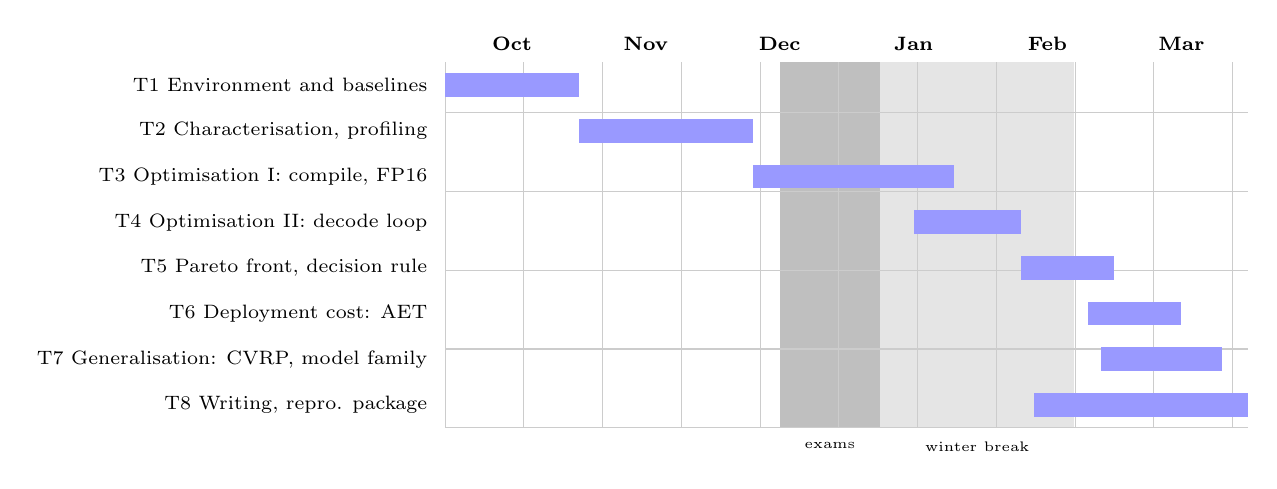
\begin{tikzpicture}[x=0.85cm, y=0.58cm, font=\scriptsize]

% low-activity periods: examinations (darker), then winter break (lighter)
\fill[black!25] (5,0) rectangle (6.5,8);
\fill[black!10] (6.5,0) rectangle (9.4,8);

% grid
\draw[black!20] (0,0) grid (12,8);

% month headers
\foreach \i/\m in {0/Oct,2/Nov,4/Dec,6/Jan,8/Feb,10/Mar} {
  \node[anchor=south, font=\scriptsize\bfseries] at (\i+1,8.05) {\m};
}

% task labels
\foreach \k/\lab in {%
  0/{T1~Environment and baselines},%
  1/{T2~Characterisation, profiling},%
  2/{T3~Optimisation I: compile, FP16},%
  3/{T4~Optimisation II: decode loop},%
  4/{T5~Pareto front, decision rule},%
  5/{T6~Deployment cost: AET},%
  6/{T7~Generalisation: CVRP, model family},%
  7/{T8~Writing, repro. package}}
  \node[anchor=east] at (-0.12, 7.5-\k) {\lab};

% bars
\foreach \k/\xa/\xb in {%
  0/0/2.0, 1/2.0/4.6, 2/4.6/7.6, 3/7.0/8.6,%
  4/8.6/10.0, 5/9.6/11.0, 6/9.8/11.6, 7/8.8/12.0}
  \fill[blue!40] (\xa,7.24-\k) rectangle (\xb,7.76-\k);

% annotations
\node[anchor=north, font=\tiny, align=center] at (5.75,-0.10) {exams};
\node[anchor=north, font=\tiny, align=center] at (7.95,-0.10) {winter break};

\end{tikzpicture}
\caption{Six-month project plan. Shaded bands mark periods of reduced
availability: examinations (mid December to early January, darker) and the winter
break that follows (to late February, lighter).}
\label{fig:gantt}
\end{figure}

\noindent\textbf{Scheduling constraints.}

\begin{itemize}[leftmargin=1.3em]

\item \textbf{Reduced availability.} Two windows are shaded in
Figure~\ref{fig:gantt}: examinations, mid December to early January, and the
winter break that follows, to late February.

\item \textbf{Tasks that overlap them.} T3, T4, part of T5 and the drafting
strand of T8 are the least machine-intensive of the project --- analysis,
ablation and writing, which tolerate interruption. The uninterrupted profiling
sweeps and thermal measurements of T2, T6 and T7 fall outside both windows.

\item \textbf{Contingencies.} Energy measurement requires a Linux environment for
per-process attribution; failing that, the AET half of O5 is deferred and the rest
of the project is unaffected. If the larger batch and instance sizes of T7 exhaust
GPU memory, the affected configurations are recorded as a reported boundary rather
than a failed run --- the memory ceiling is itself a deployment result.

\end{itemize}

%=============================================================================
\bibliographystyle{abbrvnat}
\bibliography{references}

\end{document}
